%% main.tex -- "From Lagging to Leading: The Measured Emergence of Standing
%% Capacitance Behind Consumer Connections, 1997--2025"
%% (v5 identity per V5_RESTRUCTURE_SPEC_20260807.md: the measured identification
%%  of a new term -- trajectory -> decomposition -> load-independence ->
%%  connection scaling -> labelled EMC-filter hypothesis -> implications.)
%%
%% D. J. Hume, Electricity Authority (EA hat; descriptive, not policy advocacy).
%% Self-published under CC0 1.0 as a Zenodo record with a DOI. Venue decision
%% 26 Aug 2026 (SELF_PUBLISH_PLAN_20260826.md): no journal, no submission, no
%% page cap. This file is the SHORT VERSION; the extended version is the
%% complete record. IEEEtran is retained as the typeset class only.
%%
%% Single source of truth for every number and figure: ../replication/ .
%% If a figure or number changes, change it in the replication notebooks first,
%% re-run, and it flows here (figures are pulled from ../replication/figures/).
%%
%% Build:  pdflatex main && bibtex main && pdflatex main && pdflatex main
%% (IEEEtran.cls and IEEEtran.bst are bundled in this directory.)

\documentclass[journal]{IEEEtran}

\usepackage{graphicx}
\usepackage{amsmath}
\usepackage{amssymb}
\usepackage{booktabs}
\usepackage{array}
\usepackage{url}
\usepackage[hyphens]{xurl}
\usepackage{orcidlink} % renders the ORCID iD icon; pulls in hyperref + tikz

% Figures live in the replication package (the single source of truth) and,
% as a fallback, in a local figures/ copy.
\graphicspath{{../replication/figures/}{figures/}}

\begin{document}

\title{From Lagging to Leading: The Measured\\
Emergence of Standing Capacitance Behind\\ Consumer Connections, 1997--2025}

\author{D.~J.~Hume~\orcidlink{0009-0006-6920-0598}%
\thanks{D. J. Hume is with the Electricity Authority, Wellington, New Zealand
(e-mail: corresponding author details on submission).
ORCID iD: \url{https://orcid.org/0009-0006-6920-0598}.}%
\thanks{This is descriptive analysis of public regulatory metering and
information-disclosure data. The views expressed are the author's. No external
funding was received. The analysis informs, but does not advocate, a live
reactive-power pricing policy question (Section~VI-C).}%
\thanks{Reference~\cite{hume_extended} is the \emph{extended version} of this
paper, with the analysis notebooks that compute every number and figure here from
public data: the measurement-error analysis, the churn, correspondence and
contamination screens, each method's robustness batteries and sensitivities, and
the dated regulatory arc. It is cited below at each point its material is used,
and not described again.}}

\markboth{From Lagging to Leading --- short version}%
{Hume: The Measured Emergence of Standing Capacitance Behind Consumer Connections}

\maketitle

\begin{abstract}
Both ENTSO-E Final Reports on the 2025 Iberian and North Macedonian blackouts read the excess capacitive reactive power as a network term---the reading the available data supports. The Iberian report asks for what was missing: information on load composition. We build that record from regulatory half-hourly metering at New Zealand's transmission--distribution
boundary, spanning 29 years, and find a second source: the demand behind the
customer's connection, at mains voltage and in residential, commercial and
industrial premises alike, has itself moved capacitive. Overnight reactive
power crossed from lagging to leading in 2016, nearly a decade before the 2025
events, and a first-principles charging calculation puts the demand-side share
of that drift in the physical band 75--88\%. That term behaves as a net standing shunt
element---present around the clock, scaling with the connections served, and
moving capacitive by about 230~VAr per connection over 2013--2025 and roughly
20~VAr a year at the close. It drives the drift rather than the level: the
distribution network's own cable and line charging remains the larger part of
the standing leading reactive power, and what changed is that a demand once
strongly lagging stopped masking it. The candidate device layer is the
electromagnetic-compatibility filter mandated in nearly every mains-connected
product (a labelled hypothesis): a few VAr per device, tens of devices per
household, millions across a system and perhaps billions on the
largest---permanently across the mains and switched by nobody. Its injection
rises with the square of mains voltage, so every 230-volt system accumulates about three times more per device than a 120-volt, 60-hertz one. Planning and protection studies still carry a constant
lagging load archetype, where the overnight flow now has the opposite sign.
Both inputs to the measurement are records any operator already holds.
\end{abstract}

\begin{IEEEkeywords}
Reactive power, power factor, overvoltage, load modeling, power distribution,
power system measurements.
\end{IEEEkeywords}

% ======================================================================
\section{Introduction}
% ======================================================================
\IEEEPARstart{P}{ower} systems internationally are shifting from net-absorbing
(lagging) toward net-generating (leading) reactive power at light load, as the
connected load fleet modernises toward power-electronic devices and networks add
underground cabling. The direction is not in dispute, and this paper does not
claim to be the first to observe it. What has been missing is a long
\emph{measured} record of the transition at supply-point resolution, and a
measured separation of how much of the drift is the load fleet and how much is
the network. This paper supplies both for a single national system, connects the
result to a failure mode that has recently moved from theory to realised
blackouts, and closes with what the reversal implies for the analysis and
defences built for the opposite regime. The trail leads somewhere unexpected: to
the electromagnetic-compatibility filter inside practically every mains-connected
device---capacitance that one part of the regulatory apparatus drives in and no
other part counts---advanced here as a labelled hypothesis for one limb of the
measured term, with its decisive test identified.

\subsection{A global reactive transition, already observed}
The phenomenon is well attested across jurisdictions: a steep decline in reactive
demand at minimum load in Great Britain, with distribution networks beginning to
export reactive power to the transmission system~\cite{kaloudas2017}; off-peak
overvoltage episodes attributed by the French and Queensland transmission
operators to distributed generation, underground cabling, and more efficient
end-use equipment; rising capacitive export to the extra-high-voltage network in
continental Europe~\cite{tazky2021}; and, at device level, a majority of modern
household appliances presenting a leading power factor---the jurisdiction sources
are collected in~\cite{hume_extended}. Expert reviews document the error
constant-power-factor load modelling
introduces~\cite{cigre_tb719,epri_loadmodel}. No consumer-device standard requires
a unity fundamental-frequency (displacement) power factor: IEC~61000-3-2 limits harmonic current only~\cite{iec61000_3_2}, and the one device-level power-factor
family in force anywhere (the European lighting floors~\cite{eu_lighting2020}) is
a full-load, direction-blind metric that never sees a device's standing draw. The
overvoltage-instability literature itself now records the observable: the 2026
review notes, among its causes of voltage rise, that cable substitution has
``change[d] the power factor to leading in several urban
substations''~\cite{vournas2026review}---an observation offered without citation,
and attributed wholly to the network's cables rather than to any change in what
the connected demand draws. Every system in this literature runs 230-volt mains;
Section~V-B returns to that regularity.

The closest measured system-level series is that British one: roughly eight years
(about 2005--2013) of reactive demand at grid supply points, projected forward
from load-composition modelling---neither a multi-decade measured record nor a
quantified demand-versus-network share of the realised drift, and boundary studies
elsewhere in Europe likewise characterise or simulate the export without
either~\cite{tazky2021,hume_extended}. The study closest to the present decomposition is Bosisio
\emph{et al.}~\cite{bosisio2022} on the Milan distribution network: measured
15-minute boundary data at 37 high-voltage/medium-voltage transformers, naming the
same three-term balance used here and, to our knowledge, the only prior study to
articulate this split explicitly on measured boundary data. It compares two years
across a demand shock, assigns no numerical share, and reads the dominant term as
the cables, opposite to ours; we treat it as complementary, and it leaves the
national, multi-decade, quantified attribution open~\cite{hume_extended}.

\subsection{The realised risk}
In 2025 two power systems suffered major blackouts whose official investigations
found a leading-reactive/overvoltage mechanism at their core: the Final Reports
of the European Network of Transmission System Operators for Electricity
(ENTSO-E), both published 2026, on the Iberian Peninsula event of 28 April
2025~\cite{entsoe_iberia} and on the North Macedonia event of 18 May
2025~\cite{entsoe_nm}, detailed in Section~VI-C. What matters here is what those
investigations could not do. Both treat the capacitive surplus as a network-side
quantity and low demand as a magnitude rather than as a fleet whose reactive
character has itself changed. The Iberian expert panel models the reactive response of load to voltage, but its load model's reactive voltage exponents come from a
table of typical values by load class---how the reactive power of demand varies
with voltage, not what it was---and the North Macedonian report carries no load
power-factor assumption at all; neither states the aggregate reactive character of demand anywhere~\cite{hume_extended}. The Iberian panel names the gap itself: modelling the transmission--distribution interfaces accurately would need ``information on load composition''~\cite{entsoe_iberia}. These are not criticisms of investigations that reasoned from
the data available to them; they identify the space a long measured record can
fill. The field's current synthesis has the same shape: the 2026 mechanisms
review~\cite{vournas2026review} gives as its causes of voltage rise corridors
below surge-impedance loading, cable substitution, synchronous-generator
decommissioning, and fixed-power-factor converter operation---network and
generation throughout---representing load as lagging or unity power factor in
every model, citing no measurement of demand reactive character.

\subsection{Contribution}
The contribution is layered. \emph{First, a measured trajectory:} using
regulatory half-hourly active and reactive power at New Zealand grid exit points,
we measure the system's reactive character at supply-point resolution over 29
years (1997--2025) on a balanced panel---the same grid exit points in every year,
so sites entering or leaving the record cannot manufacture the trend---and show
the drift is a property of the system rather than of its metering. The computation reuses settlement metering that any operator holds, so the same
measurement is available to any system.

\emph{Second, a decomposition of the drift} into a demand-side load-composition
component and a distribution network cable-charging component. The magnitude is carried by a
first-principles charging calculation that computes each network's cable charging
directly from its disclosed circuit kilometres and so fits no cable coefficient;
over the 2013--2025 disclosure window it puts the demand-side (\emph{organic})
share at about 80\% (physical band 75--88\%), with two statistical methods
corroborating the direction but not themselves pinning the share.

\emph{Third, the term identified.} The deepening is load-independent---as large
at the flat evening peak as overnight---so it behaves as a standing shunt
element, permanently energised, rather than as a change in how the load draws
reactive power while operating; and it lives behind the connections, the
2013--2025 deepening being proportional to the number served with no detectable
connection-independent residual, at about 230~VAr per connection (Section~V);
split by the registry's consumer classes, the residential connections---which
hold no power-factor-correction plant---carry the smaller coefficient of
the two. We
advance the mandated electromagnetic-compatibility filter capacitance as its
candidate device layer (a labelled hypothesis) and identify the decisive
low-voltage measurement that would settle it.

The significance is what the reversal does to analysis: the direction of the
binding voltage-security question reverses; the automatic last-resort defences
and the margin tooling of the undervoltage era do not transfer; and the
constant-lagging-power-factor load archetypes of planning and protection studies
no longer describe the light-load fleet (Section~VII)---a qualitative synthesis,
not a defence-scheme or load-model redesign.

This work extends the author's EEA~2025 conference paper~\cite{hume2025}, which
described the 2009--2024 aggregate trend qualitatively, by adding the 1997
baseline, grid-exit-point resolution, the artefact test, the decomposition and the
connection-scaling identification.

% ======================================================================
\section{Data and Method}
% ======================================================================
\subsection{Sign convention and primary variable}
Reactive power carries a direction that is the entire point of this study. We
use the convention $Q<0$ for \emph{leading} (capacitive, voltage-raising) and
$Q>0$ for \emph{lagging} (inductive, voltage-lowering), and lead throughout with
the signed reactive power in MVAr, which is additive across supply points and has
no discontinuity at unity, and present power factor only as a familiar
comparator (load convention; the generator convention reverses both signs). Power factor is non-additive, so where a system power
factor is quoted we sum $P$ and $Q$ across the panel first and derive
$\mathrm{PF}=\Sigma P/\sqrt{(\Sigma P)^2+(\Sigma Q)^2}$.

\subsection{The grid-metering record and the balanced panel}
The primary data is half-hourly real and reactive power at every grid exit point
(GXP), the substations where the national transmission grid hands electricity to
the local distribution networks, from 1997 to 2025, published by the New Zealand
Electricity Authority on its Electricity Market Information (EMI) platform. Over
the record, 238 distinct GXPs appear; a balanced core of 132 is present in all 29
years. The reactive column has been recorded for twenty-nine years because
settlement metering records it, not because it was the object of anyone's
question: the centralised data set was assembled for demand forecasting and the
Grid Investment Test.

We reduce each GXP's year to a small set of features, of which the headline
quantities are the average overnight and evening-peak reactive and real power.
The overnight window is trading periods 6--10 (approximately 02:30--05:00, the
lowest demand) and the evening peak is trading periods 36--38 (approximately
17:30--19:00); we also record the fraction of overnight half-hours that were
leading.

The largest way a 29-year trend could be spurious is a change in the set of
measured GXPs: new urban, cable-heavy sites appearing and old rural ones dropping
out would manufacture a leading trend from bookkeeping alone. The defence is the
\emph{balanced panel} of the 132 GXPs present in every one of the 29 years, so any
change is a change in the same sites rather than in which sites are measured. The panel is churn-controlled by construction (``balanced'' in the panel-data
sense, not the three-phase sense), and we follow one rule throughout:
\emph{trends on the balanced panel, snapshots on the full panel}. Restricting it
to demand networks leaves 123 GXPs; the 132-point and 123-point figures are
reported distinctly and kept labelled throughout.
The residual bias is signed: the demand grid exit points excluded from the panel
are by 2025 on average \emph{more} leading than it and drift faster, so the
balanced panel, if anything, understates the national drift~\cite{hume_extended}. Five national totals follow, each on the sample its method requires, and Table~\ref{tab:panels} sets them side by side. They differ by sample, window and summary statistic rather than by measurement; a reader wanting one figure for New Zealand should take the first row.

\begin{table}[!t]
\caption{The National Overnight Totals, and the Sample Each Comes From}
\label{tab:panels}
\centering
\renewcommand{\arraystretch}{1.18}
\begin{tabular}{@{}>{\raggedright\arraybackslash}p{0.31\columnwidth}>{\raggedright\arraybackslash}p{0.16\columnwidth}>{\raggedright\arraybackslash}p{0.37\columnwidth}@{}}
\toprule
\textbf{Sample} & \textbf{Window} & \textbf{Overnight reactive power} \\
\midrule
Balanced demand panel, 123 GXPs \emph{(the headline)} & 1997--2025 & $+466 \rightarrow -451$~MVAr \\
Balanced full panel, 132 GXPs & 1997--2025 & $+673 \rightarrow -296$~MVAr \\
Clean and clean-strict cohorts, 119 and 92 GXPs & 1997--2025 & about $-300$~MVAr in 2025 \\
Charging footprint, 29 networks & 2013--2025 & $-541$~MVAr in 2025, drifting $-49.9$~MVAr/yr \\
Connection-scaling panel, 114 GXPs & 2013--2025 & $+188 \rightarrow -182$~MVAr (medians) \\
\bottomrule
\end{tabular}
\end{table}

\subsection{Metering provenance and accuracy}
The active and reactive power at each grid exit point is settlement-grade revenue
metering in the highest-accuracy category of the regulatory Metering
Code~\cite{eipc_part10}: Class~0.2S for active energy under IEC~62053-22~\cite{iec62053_22}, with the reactive channel held to the looser Class~2--3 of IEC~62053-23~\cite{iec62053_23}, and the metered quantity is the
fundamental-frequency (\emph{displacement}) reactive power of IEEE Std~1459~\cite{ieee1459}. Random error averages down under aggregation and cannot
manufacture a near-monotonic 900-MVAr swing through zero; the one systematic
error that does not average down---a phase displacement $\beta$ in the
instrument-transformer chain, injecting a spurious term of about $P\sin\beta$
that matters most in exactly the light-load window this paper measures---is bounded,
under a common-mode half-degree assumption, at some fifty times smaller than the
swing. That bound does not rest on the half degree. A \emph{static} displacement generates apparent drift only through the growth of the load it multiplies, so the most it can produce across the whole record is $\Delta P\sin\beta$; overnight panel load grew by $\Delta P=280$~MW and $\sin\beta\leq1$, so a static displacement of any size---$90^\circ$ on every transformer set included---falls three times short of the swing. The stronger defence: it is largest in the loaded window while the
deepening is near-equal in both (Section~V-A). The full measurement-error analysis is in~\cite{hume_extended}; we therefore treat the multi-decade \emph{drift} as
robust while regarding the standing reactive \emph{level} on any single night as
carrying a bounded measurement uncertainty.

\subsection{The asset (parameter) record}
To describe each network's physical make-up we assemble a per-company, per-year
table from the Commerce Commission's regulated information disclosures: circuit
length split into overhead and underground kilometres at each operating voltage
(Schedule~9c, disclosed consistently from 2013), capacitor-bank counts
(Schedule~9a), demand and connection counts and embedded generation (Schedule~9e), and the regulated
asset base (Schedule~4). The disclosures are mapped to the EMI network codes
through a 29-year validated correspondence, time-aware because ownership itself
changed under the record~\cite{hume_extended}. Two data-quality choices matter here: only
``All''-network roll-up rows are retained, and the capacitor series, counts only
and carrying a 2014--2015 definitional break, is used as a direction-only proxy.

\subsection{Confounds in the metered reactive power}
A grid exit point meter records the \emph{net} reactive power at the boundary, which
is not in general a clean distribution offtake:
\begin{equation*}
Q_{\text{metered}} = \underbrace{Q_{\text{load}} + Q_{\text{cable}}}_{\text{the subject of this paper}}
\;-\; Q_{\text{embedded gen}} \;\pm\; Q_{\text{TP plant}},
\end{equation*}
where the last two terms are \emph{confounds}: other reactive sources mixed
into the same metered reading. An embedded
\emph{synchronous} generator sets its reactive output by the voltage it sees
rather than by local load; and at some substations Transpower voltage-regulating
plant shares the substation with the offtake, with the revenue-metering boundary
determining whether it registers in the metered flow. One behavioural diagnostic catches all of
these, whichever party owns the plant: a clean distribution offtake's reactive
power tracks its load, so a straight-line fit of $Q$ on $P$ explains an appreciable
share of its variation ($R^2 \approx 0.3$--$0.5$), whereas voltage-regulated reactive
is decoupled ($R^2 \to 0$). Computed on three spread-out years (2016, 2019, 2022)
so that a flag reflects a stable trait, it isolates six \emph{decoupled}---that is,
\emph{contaminated}---grid exit points at Christchurch, Auckland, Bunnythorpe and
Tuai~\cite{hume_extended}.

This matters overnight specifically: the minimum removes generation that merely
stops, leaving plant that regulates voltage around the clock---synchronous
machines, and increasingly inverter-based plant running a night-time reactive mode
at zero active power. We flag such sites rather than discard them silently, and
Sections~III-B and IV show the trajectory and the decomposition robust to their
removal: the contamination moves the absolute \emph{level}, not the direction,
intensity or attribution of the drift.

\subsection{Analysis methods}
The trajectory is summarised by ordinary linear slopes for headline rates and, for
robustness, by Theil--Sen slopes~\cite{sen1968}, which a few anomalous years cannot
move; where the two agree---as they do throughout---a trend rests on no small set
of years. The metering-artefact test (Section~III-B)~\cite{hume_extended} removes
each GXP's own Theil--Sen trend and looks in what remains for a step shared across
sites in the same year.

% ======================================================================
\section{The 29-Year Reactive Trajectory}
% ======================================================================
\subsection{Lagging to leading, overnight}
Fig.~\ref{fig:traj} shows the central empirical result. Summed across the
balanced demand panel, mean overnight reactive power fell from $+466$~MVAr
(lagging) in 1997 to $-451$~MVAr (leading) in 2025, a near-monotonic linear drift
of $-31.1$~MVAr/yr (robust Theil--Sen slope $-31.3$~MVAr/yr, 95\% confidence
interval (CI) $[-34.0,-28.1]$~\cite{sen1968}---the spread among the pairwise
slopes, not a coverage guarantee, since consecutive years are not independent), crossing into net-leading overnight in
2016. On the wider 132-point balanced panel, which also includes
non-distribution connection points, the same drift reads
$+673\rightarrow-296$~MVAr at $-30.3$~MVAr/yr, crossing in 2020. Expressed per megawatt of overnight load, the drift is about
$-0.018$~MVAr/MW/yr. In the comparator of
Section~II-A, the overnight aggregate power factor moved from 0.964 lagging to 0.975
leading---a small excursion either side of unity concealing a 900-MVAr reversal,
which is why signed reactive power is the working variable throughout.

\begin{figure}[!t]
\centering
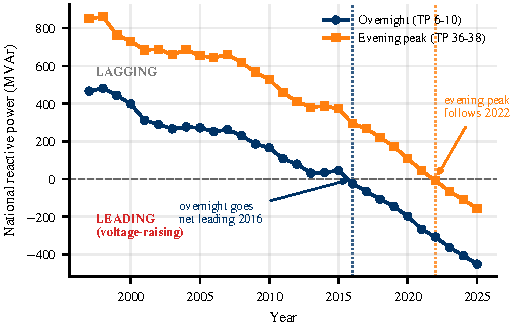
\includegraphics[width=\columnwidth]{01_trajectory_journal.pdf}
\caption{The 29-year reactive trajectory on the balanced demand panel of 123
grid exit points, overnight against the evening peak ($Q<0$ is leading).}
\label{fig:traj}
\end{figure}

The diurnal contrast is itself a result. The evening peak crossed net-leading
only in 2022 and remains far less leading than overnight, which locates the
net-leading regime firmly at low load. Expressed as a fraction rather than a sum,
the mean share of overnight half-hours that are leading rose from about 1\% in
1997 to about 74\% in 2025.

\subsection{A measured property, robust to contaminated sites}
A measurement artefact cannot reproduce the trend's physical structure. The
net-leading crossing is specific to the overnight window---the evening peak stays
lagging for years longer (Fig.~\ref{fig:traj})---while the deepening beneath the
crossings is near-equal in the two windows over 2013--2025, with evening-peak
load essentially flat (Section~V-A): the signature of a standing capacitive term
netted against different amounts of lagging load. The drift also tracks each
network's underground-cable intensity and grows with each grid exit point's
connection count, neither of which a metering error has a reason to do. It does
not rest on the older, less homogeneous early data, it is not seasonal, and, since a single system-wide re-base would step every supply point at once, a separate test finds no such event~\cite{hume_extended}. The lagging-to-leading drift is therefore
a measured property of the system, not an artefact of how it was metered.

The trend could also be carried by a few grid exit points whose meters do not see
a clean distribution offtake (Section~II-E), so we test it by removing them:
the six \emph{decoupled} points, leaving the \emph{clean} cohort, and more strictly the
steady-generation and net-export points too (\emph{clean-strict}). The absolute
total and the MVAr/yr slope \emph{shrink}---the 2025 total from $-451$ to about
$-300$~MVAr, the slope from $-31.1$ to $-23.4$~MVAr/yr---because two removed nodes
carry large, load-decoupled leading values. The per-MW drift intensity, by
contrast, is essentially unchanged ($-0.0175$, $-0.0178$, and
$-0.0180$~MVAr/MW/yr across the full, clean, and clean-strict cohorts), and the
share of networks net-leading overnight by 2025 is likewise stable (75\%, 74\%,
80\%). The phenomenon's intensity per unit load and its near-universal reach do
not depend on the contaminated nodes; only the headline \emph{size} does.

% ======================================================================
\section{Decomposition: Demand vs Network}
% ======================================================================
The policy-relevant question is how much of the drift is the network's own cables,
which inject leading reactive power as a distributed capacitance, and how much is
the changing make-up of demand itself: the retreat of inductive plant and the
accumulation of power-electronic equipment (LED lighting, switch-mode supplies,
heat pumps and other variable-speed drives). We call the second part
\emph{organic}: it is in the load fleet, not the wires. Mostly cables would make
it a familiar network-planning problem; mostly the demand fleet makes it
structural, nationwide, and outside any single network's control. We approach it three ways; the two statistical methods
share a common underground-cable proxy, while the physics-based method fits no
cable coefficient and is independent of both.

\subsection{Method 1: a clean-cohort contrast}
Some distribution businesses are almost entirely overhead line, which injects
little leading reactive power, so if their overnight reactive power still drifts
leading, that drift can only be the demand fleet. We compare reactive power per MW of load
(so network size cancels), load-weighted within each cohort, for networks at or
below 12\% underground (\emph{clean} in this method's sense) against those at or
above 40\% (cable-rich).

The clean cohort drifts from $+0.373$ to $+0.065$~MVAr/MW (slope $-0.0101$/yr),
ending near balanced; the cable-rich cohort drifts from $+0.205$ to
$-0.306$~MVAr/MW (slope $-0.0134$/yr), crossing well into leading. The ratio of
slopes puts the demand-side share of the cable-rich cohort's drift at about 75\%.
The reading rests on two assumptions: that the organic per-MW drift is common
across the cohorts (to the extent urban fleets modernise faster, the cable share
is overstated), and that the at-most-12\%-underground cohort carries no material
cable term (to the extent it does, the demand share is overstated); the two pull
in opposite directions. The exact ratio also moves with measurement choices,
spanning the 64--90\% collected in Table~\ref{tab:triangulation}; each variant is worked in~\cite{hume_extended}.

The \emph{direction} is therefore robust while the \emph{exact ratio} is not,
which is why we treat Method~1's ratio as a hypothesis and bring two further
methods. And although cable is the minority of the drift, it is the marginal
factor that tips a network from balanced into net-leading, so cable intensity
shapes \emph{where} overvoltage appears first even though demand composition
drives the trend.

\begin{figure}[!t]
\centering
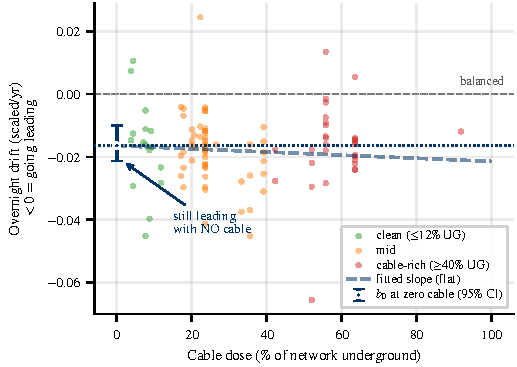
\includegraphics[width=\columnwidth]{02_dose_response_journal.pdf}
\caption{Method~2, the dose-response: each grid exit point's overnight reactive
drift, scaled by its own typical size, against its network's cable dose.}
\label{fig:dose}
\end{figure}

\subsection{Method 2: a validated dose-response}
The second method asks whether the networks with more cable drift faster. Each
GXP is reduced to one number---the Theil--Sen slope of its overnight reactive
power, scaled by its own typical size---and those per-site drifts are then fitted
against the site's \emph{cable dose}, the percentage of its network that runs
underground. The line has two coefficients, and only one of them is this
paper's result. At zero cable there is no cable charging, so any drift remaining
at that end of the line must come from the demand: the intercept $b_0$ is the
organic drift. The slope $b_1$ is the extra drift per added point of
underground---the cable contribution. Fig.~\ref{fig:dose} shows both.

Two features of the fit follow from how the dose is recorded. Cable dose is a
property of the \emph{company}, so every site in a network carries the identical
value and the sites are not independent. The model therefore lets each company
sit at its own baseline (a random intercept), and the uncertainty comes from a
\emph{cluster bootstrap}: the fit is repeated on thousands of datasets drawn at
random, with replacement, from the data itself, and the reported interval is the
spread of those answers---drawing whole companies rather than single sites, so
that the dependence is carried into the interval.

Before any use on the real data the estimator was validated on synthetic panels
with planted answers. It recovers $b_0$ reliably. It recovers the organic
\emph{share} only when the cable effect is itself identified, and the reason is
arithmetic: that share is $b_0/(b_0+b_1 d)$ at dose $d$, which puts $b_1$ in the
denominator. On the real data $b_1$ is not identified, so the share cannot be
pinned even though $b_0$ is---and the magnitude falls to Method~3.

On the real data, the organic drift is $b_0=-0.016$/yr (95\% CI
$[-0.021,-0.010]$), leading in 100\% of bootstrap resamples. The cable slope is
$b_1=-0.00005$/yr (95\% CI $[-0.00037,+0.00012]$), which crosses zero---weakly
identified, because cable dose is a company-level trait with only about 23
distinct values---so we deliberately publish no tight interval on the share (at
the point estimate it is at least 78\%, consistent with 100\%, which is
an arithmetic consequence of an unpinned denominator rather than a result;
Table~\ref{tab:triangulation}). Three further checks hold~\cite{hume_extended}: adding capacitor intensity as a control moves $b_0$ about 10\%; cable dose and distributed-generation intensity are weakly correlated ($-0.22$); and restoring the four sites dropped in the mapping moves $b_0$ under 1\%.

A fourth check replaces the dose measure altogether: refitting with each
network's computed charging intensity as the dose---Method~3's physical $\omega C
V^2 \ell$ per MW of maximum demand---moves $b_0$ only from $-0.0164$ to
$-0.0178$/yr. The two dose measures are in fact \emph{negatively} correlated
across networks ($r=-0.23$), so two nearly opposite dose definitions returning
the same organic conclusion is a stronger robustness statement than either alone.
No reading here rests on the cable slope under either dose.

\subsection{Method 3: first-principles charging physics}
The third method computes the network contribution directly from physics, with no
fitted coefficient, so it sidesteps the weak-identification problem entirely. Any
energised length of cable or line behaves as a distributed capacitance and
injects a fixed leading reactive power $Q=\omega C V^2 \ell$, with $C$ the
capacitance per km, $V$ the operating voltage, and $\ell$ the length. Using the
published overhead and underground kilometres at each voltage from Schedule~9c
(Section~II-D), textbook per-km capacitances with an explicit $\pm 35\%$ band
carried through to the result, and a band-by-band sum, we compute the physical charging per network
per year and subtract it from the measured overnight reactive power; the
remainder is organic. The band voltage is nominal and held across the record;
three-quarters of the computed charging sits at or below 33~kV, where the tap
changer holds voltage to a target, and a sustained 4\% rise across the window
would be needed to carry the organic share out of the physical band
below~\cite{hume_extended}. That remainder is a residual, and we name the principal further terms it
absorbs: transformer magnetising reactive power, series-reactance absorption, and
the distribution capacitor fleet (static-to-shrinking, Section~VI-B). Each is either second-order overnight or biases the residual toward lagging, so
reading it as the demand-side drift is conservative. The footprint carries no
decoupled-node screen, so embedded generation sits in the residual too; re-running
the decomposition without those sites moves the organic share \emph{up} rather
than down~\cite{hume_extended}.

Over 2013--2025 the measured overnight reactive power drifts at $-49.9$~MVAr/yr
across all demand networks, of which the physical charging contributes only
$-9.2$~MVAr/yr and the organic residual $-40.7$~MVAr/yr. The organic share of the
\emph{drift} is therefore about 80\% (physical band 75--88\%), and because this
method fits no cable coefficient it is independent of the two statistical
methods. The window is set by the data: the disclosed circuit kilometres are
recorded consistently only from 2013, so extending the $\sim$80\% share to the
full 29 years is an inference, not a second measurement. This all-network
footprint rate is a different sample from the balanced panels of Section~III, and the only
one of this paper's three drift rates that carries the organic share.

The composition of the leading reactive power \emph{standing on the network
today}---the level, as opposed to the drift---is a separate and weaker claim, and
on it the physics points the other way: a large, near-static charging baseline has
always been present, and what changed is that the organic demand crossed from
lagging, which masked it, to leading, which does not. We quote no precise level
share, and carry the reading qualitatively into Sections~VI and VII.

\begin{figure}[!t]
\centering
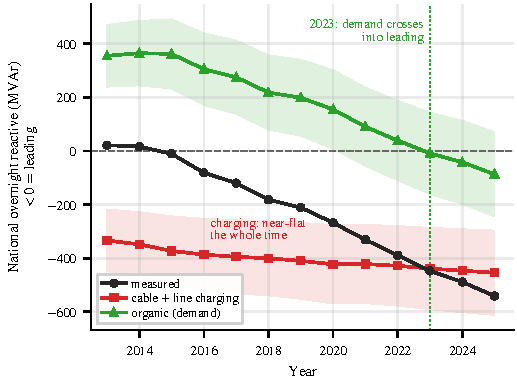
\includegraphics[width=\columnwidth]{03_level_journal.pdf}
\caption{Measured overnight reactive power across all demand networks (black) against its two components, cable and line charging (red) and the organic demand term (green). Bands are the $\pm 35\%$ capacitance range carried through. A different
sample from Fig.~\ref{fig:traj}.}
\label{fig:level}
\end{figure}

\subsection{Triangulation}
Table~\ref{tab:triangulation} collects the three methods, which play different
roles and are not all independent: Methods~1 and 2 both rest on the same
underground-cable proxy, whereas Method~3 fits no cable coefficient at all. All
three, though, consume the same Schedule~9c circuit-length disclosures, so
agreement among them cannot diagnose a systematic kilometre error; under-counted
cable would push every method toward the demand side. A cross-sectional check
agrees: the most-leading demand grid exit points are not the most-cabled---they
sit at roughly half the cable intensity of the most-cabled group---so cable cannot be what drives the deepest-leading behaviour. The three methods share one subject---the \emph{rate} at which the overnight
reactive power moved---and Fig.~\ref{fig:level} sets it against the standing
\emph{level}. The pair carries the practical reading: the distribution network's charging is the larger part of the leading reactive power present tonight, and the demand is the larger part of why that total has moved.

\begin{table}[!t]
\caption{Three Decompositions of the Drift}
\label{tab:triangulation}
\centering
\renewcommand{\arraystretch}{1.18}
\begin{tabular}{@{}p{0.27\columnwidth}p{0.24\columnwidth}p{0.37\columnwidth}@{}}
\toprule
\textbf{Method} & \textbf{Establishes} & \textbf{Organic share of drift} \\
\midrule
1: clean-cohort contrast (cable proxy) & direction (shares the cable proxy with 2) & $\sim$75\% (78\% with contaminated nodes removed; 64--90\% across attribution, cable-intensity, and panel definitions) \\
2: dose-response (cable proxy) & direction; dominance at typical doses & $\geq$78\% at the point estimate, consistent with 100\% (cable term not pinned by the data) \\
3: charging physics (no fitted cable term) & \textbf{magnitude} & $\sim$80\% (physical band 75--88\%) \\
\bottomrule
\end{tabular}
\end{table}

% ======================================================================
\section{The Demand-Side Term Identified: A Standing Shunt Term Behind
Connections}
% ======================================================================
The decomposition attributes the drift to the demand fleet; it does not say what
in the fleet is doing it. Two measured properties narrow the answer, a specific
physical candidate follows from them, and a scaling test probes the candidate's
sharpest prediction.

\subsection{Load-independent, around the clock}
First, the drift is load-independent. Over the 2013--2025 window we summarise
each grid exit point passing the full contamination screen by robust annual
medians on wider windows than the Section~II features. On the 114 such grid exit
points with both endpoints metered, the median per-site change in reactive power
is $-2.25$~MVAr overnight and $-2.42$~MVAr at the evening peak (median per-site
ratio 1.06), while evening-peak load was essentially flat (median change
$+2.9\%$). A change in how the connected load draws reactive power while
operating would scale with the load operating---far larger at the peak than at
03:00---and so would the load-proportional metering bias bounded in
Section~II-C. A near-equal deepening around the clock is instead the signature of a
\emph{standing shunt term}: always energised, indifferent to what the load
is doing. It also reconciles the diurnal structure of Fig.~\ref{fig:traj}, since
net-leading surfaces overnight first because the standing component is netted
against more lagging load at the peak.

What the test identifies is the \emph{net} standing term. A standing shunt
inductance is load-independent and scales with $V^2$ exactly as a capacitance does,
so the record returns the difference of two limbs and never either one---and both
moved across the window. Filter-carrying electronics accumulated; the permanently
energised magnetics retreated, in linear transformer supplies, overnight magnetic
ballasts, always-on shaded-pole motors, and the distribution transformer's own
magnetising reactive power, itself standing, connection-scaling and
inductive~\cite{hume_extended}. A retirement moves the net exactly as an addition
does. We report the net term throughout, and read the device layer below as a
candidate for its capacitive limb alone.

\subsection{A physical candidate: the mandated EMC filter}
Second, the term must live behind essentially every connection, because
the drift's reach is near-universal across grid exit points. We therefore advance
a specific physical candidate, labelled plainly as a hypothesis: the
electromagnetic-compatibility (EMC) filter that practically every mains-connected
electronic product is required to carry. A switched-mode device chops current at
tens to hundreds of kilohertz, and conducted-emission limits (the international CISPR~32 limits~\cite{cispr32}, a condition of sale in most jurisdictions, New
Zealand included) oblige its manufacturer to stop that noise at the appliance's
own terminals; the universal compliance solution is a passive filter directly
across the mains input (Fig.~\ref{fig:emifilter}). Its elements carry safety-class
names from where they connect: \emph{X-capacitors} bridge line
and neutral, the one position where a capacitor is permitted to be large
(typically 0.1--2.2~$\mu$F), because a short circuit there is an overcurrent
event the fuse clears rather than a shock hazard; \emph{Y-capacitors} run to
earth and are held to nanofarads by touch-current limits.

\begin{figure}[!t]
\centering
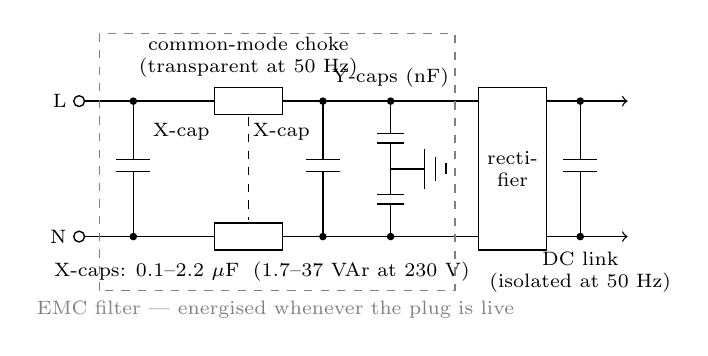
\begin{tikzpicture}[x=0.86mm, y=0.86mm, line width=0.5pt, font=\scriptsize]
% mains terminals and rails
\draw[fill=white] (2,20) circle (0.8) node[left=1pt] {L};
\draw[fill=white] (2,0) circle (0.8) node[left=1pt] {N};
\draw (2.8,20) -- (22,20);
\draw (2.8,0) -- (22,0);
% X1 capacitor
\draw (10,20) -- (10,11.4);
\draw (7.5,11.4) -- (12.5,11.4);
\draw (7.5,9.6) -- (12.5,9.6);
\draw (10,9.6) -- (10,0);
\filldraw (10,20) circle (0.45); \filldraw (10,0) circle (0.45);
\node[right=2pt] at (10.6,15.5) {X-cap};
% common-mode choke
\draw (22,18) rectangle (32,22);
\draw (22,-2) rectangle (32,2);
\draw[dashed] (27,17.6) -- (27,2.4);
\node[align=center] at (27,26.5) {common-mode choke\\(transparent at 50~Hz)};
\draw (32,20) -- (58,20);
\draw (32,0) -- (58,0);
% X2 capacitor
\draw (38,20) -- (38,11.4);
\draw (35.5,11.4) -- (40.5,11.4);
\draw (35.5,9.6) -- (40.5,9.6);
\draw (38,9.6) -- (38,0);
\filldraw (38,20) circle (0.45); \filldraw (38,0) circle (0.45);
\node[left=2pt, fill=white, inner sep=1pt] at (37.4,15.5) {X-cap};
\node[align=center, fill=white, inner sep=1pt] at (29,-5.2) {X-caps: $0.1$--$2.2~\mu$F\; ($1.7$--$37$~VAr at 230~V)};
% Y capacitors to earth
\draw (48,20) -- (48,15.2);
\draw (46,15.2) -- (50,15.2);
\draw (46,13.8) -- (50,13.8);
\draw (48,13.8) -- (48,10);
\draw (48,0) -- (48,4.8);
\draw (46,4.8) -- (50,4.8);
\draw (46,6.2) -- (50,6.2);
\draw (48,6.2) -- (48,10);
\filldraw (48,20) circle (0.45); \filldraw (48,0) circle (0.45);
\draw (48,10) -- (53,10);
\draw (53,13) -- (53,7);
\draw (54.6,11.8) -- (54.6,8.2);
\draw (56.2,10.8) -- (56.2,9.2);
\node at (48,23.5) {Y-caps (nF)};
% filter boundary
\draw[dashed, gray] (5,-8) rectangle (57.5,30);
\node[gray] at (31,-10.8) {EMC filter --- energised whenever the plug is live};
% rectifier and DC link
\draw (58,20) -- (61,20); \draw (58,0) -- (61,0);
\draw (61,-2) rectangle (71,22);
\node[align=center] at (66,10) {recti-\\fier};
\draw (71,20) -- (80,20); \draw (71,0) -- (80,0);
\draw (76,20) -- (76,11.4);
\draw (73.5,11.4) -- (78.5,11.4);
\draw (73.5,9.6) -- (78.5,9.6);
\draw (76,9.6) -- (76,0);
\filldraw (76,20) circle (0.45); \filldraw (76,0) circle (0.45);
\node[align=center] at (76,-5.2) {DC link\\(isolated at 50~Hz)};
\draw[->] (80,20) -- (83,20);
\draw[->] (80,0) -- (83,0);
\end{tikzpicture}
\caption{The mains input stage of a switched-mode device. Values are
datasheet-grade typical ranges, per device rather than per capacitor.}
\label{fig:emifilter}
\end{figure}

At 50~Hz the filter's only material injection is the X-capacitance, which sits
across 230~V drawing pure leading current whenever the plug is live---ahead of
the rectifier and of any standby logic. The arithmetic is $Q=\omega C V^2$, and
the fleet is one worldwide design, so the capacitance is chosen once and the
mains it lands on sets the draw: the same microfarad that injects 16.6~VAr at
230~V injects 5.4~VAr on North America's 120~V, 60~Hz mains and 3.1--3.8~VAr at
Japan's 100~V---roughly three times the standing draw per device here as in North
America, and four to five times Japan's. The accumulation is one-way: one instrument
drives the capacitance into practically every product, while none bounds its
fundamental-frequency injection at any scale, as far as we are aware~\cite{hume_extended}.

The hypothesis is narrow: the large DC-link capacitor
behind the rectifier makes no standing injection (Fig.~\ref{fig:emifilter});
motor-run capacitors sit in series with the motor's auxiliary winding and are
disconnected with it; and rooftop solar inverters contribute almost none
overnight, the isolation relay stranding the converter-side filter capacitors---a bound rather than an assumption~\cite{hume_extended}.

A bottom-up order-of-magnitude estimate---roughly two million households, each
with 20--40 permanently connected filter-carrying devices at 2--4~VAr (roughly
80--320~MVAr in aggregate), plus a commercial and industrial fleet of the same
order---puts the national standing total at roughly 150--600~MVAr, or
100--200~VAr per household as the central band. Heat pumps, an adoption jump
inside the study window, work out at roughly
37--69~MVAr~\cite{hume_extended}, of order a quarter of the
residential envelope, so the bulk belongs to the far more numerous small
supplies. The per-device values are datasheet-grade reference designs rather than
teardowns, and the device counts are estimate arithmetic anchored by intrusive
standby surveys rather than a census~\cite{hume_extended}. The estimate makes
two testable predictions: the national scale of the drift, and---because the
fleet lives behind consumer connections---that the drift should scale with the
number of connections served, with nothing left at zero connections.

The first prediction is met at the order-of-magnitude grade the estimate carries.
Summed across the same 114 grid exit points, the median overnight reactive power
moved from $+188$~MVAr (net absorbing) in 2013 to $-182$~MVAr in 2025. Those exit
points serve about 1.5~million connections---two-thirds of the national connection count---so the 369~MVAr rise normalises to about
210--280~VAr per connection~\cite{hume_extended}---above the estimate's
100--200~VAr per household centre rather than inside it, because a connection is not a household:
Section~V-C separates the consumer classes and puts the residential rate back
inside the band.

The dose arithmetic adds a third, cross-country prediction: if the filter is the
mechanism, the per-connection drift should order across systems as $\omega V^2$---Japan, then North America, then the 230-volt world---an ordering cables, heat
pumps and correction plant have no reason to reproduce. It is a test and not a
conclusion: a 120-volt supply draws twice the current for the same power and may
need \emph{more} X-capacitance, so the dose ordering holds exactly only for the
universal-input supply designed once for every market~\cite{hume_extended}. Every
system in Section~I-A runs 230-volt mains; we are not aware of an equivalent North
American measured report, an absence of measurement rather than evidence of absence. Of the two domestic predictions the second is the more
discriminating; Section~V-C tests it.

\subsection{A connection-scaling test}
Connection counts are public: the retail market-structure dataset records the
number of installation control points (ICPs---metered connections) behind each
network supply point, monthly, from December 2003~\cite{emi_icp}. We sum them to
each grid exit point and regress each panel unit's 2013--2025 change in median
overnight reactive power on the connections it serves, on the $n=96$ panel units a correspondence audit leaves, grid exit points grouped where the registry's supply-point attribution and the metering boundaries disagree. Section~V-B's estimate sets the test in advance: a
slope clear of zero, inside a per-connection band around the bottom-up figure,
and explaining a substantial share of the cross-site variance. A
grid-exit-point-level metering artefact predicts a mean-only model instead. The
criteria, the audit, and the site dispositions are in~\cite{hume_extended}.

\begin{figure}[!t]
\centering
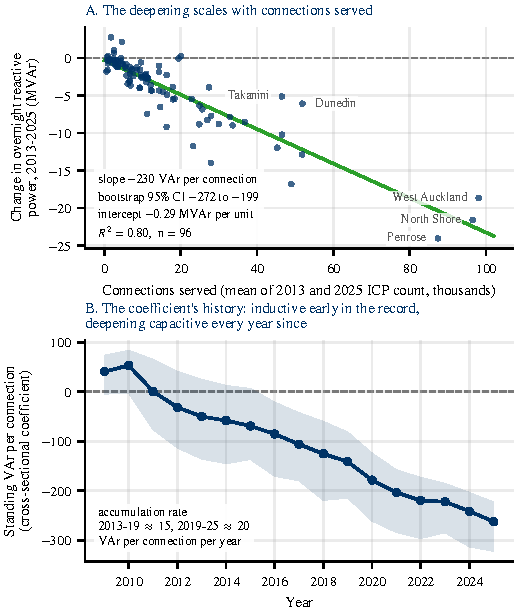
\includegraphics[width=0.94\columnwidth]{06_connection_scaling.pdf}
\caption{The connection-scaling test: (A) each panel unit's 2013--2025 change in
overnight reactive power against the connections it serves; (B) the same
coefficient refitted on each year's standing level.}
\label{fig:icp}
\end{figure}

The result is Fig.~\ref{fig:icp}: the deepening scales linearly with connections
served, at $-230$~VAr per connection, and a through-origin fit agrees ($-237$).
All three criteria are met, the mean-only artefact model loses decisively on the
standard model-selection score, and the intercept is indistinguishable from zero
under every inference scheme---so the bottom-up estimate's prediction of nothing
at zero connections is met on both limbs. Connections also beat size, the null that
matters here since both scale with it: fitted jointly against each unit's overnight
or peak real power, the connection term keeps an interval clear of zero and the
load term does not, and dropping the five highest-leverage units \emph{raises} the
coefficient to $-261$~\cite{hume_extended}.

The coefficient also has a history (Fig.~\ref{fig:icp}B). Refitted year by year
on each year's standing level, so that it carries the whole connection-scaling
class, the per-connection term starts on the \emph{inductive} side of the axis
($+41$~VAr per connection in 2009), crosses zero early in the 2010s, and reaches
$-262$~VAr per connection by 2025. The yearly intervals leave the ramp and the post-2016 deepening as what the data establish, rather than the crossing date. The 2013--2025 movement, $-212$~VAr per connection, reproduces the two-endpoint slope within 10\%.


\begin{figure}[!t]
\centering
% GENERATED by replication/src/07_anzsic_class_split.py -- do not edit by hand
\definecolor{clsall}{HTML}{4D4D4D}
\definecolor{clsres}{HTML}{003366}
\definecolor{clsci}{HTML}{D62728}
\begin{tikzpicture}[x=1mm,y=1mm,font=\scriptsize,line width=0.5pt]
\draw[black!45,line width=0.4pt] (50.96,-3.2) -- (50.96,18.20);
\draw[black!55,line width=0.4pt] (0,-3.2) -- (53.00,-3.2);
\draw[black!55,line width=0.4pt] (0.00,-3.2) -- (0.00,-4.2);
\node[below,font=\tiny,text=black!70] at (0.00,-4.2) {-1500};
\draw[black!55,line width=0.4pt] (16.99,-3.2) -- (16.99,-4.2);
\node[below,font=\tiny,text=black!70] at (16.99,-4.2) {-1000};
\draw[black!55,line width=0.4pt] (33.97,-3.2) -- (33.97,-4.2);
\node[below,font=\tiny,text=black!70] at (33.97,-4.2) {-500};
\draw[black!55,line width=0.4pt] (50.96,-3.2) -- (50.96,-4.2);
\node[below,font=\tiny,text=black!70] at (50.96,-4.2) {0};
\node[below,font=\tiny,text=black!70,align=center] at (26.50,-7.4) {VAr per connection\\(negative = added leading)};
\draw[clsall!60,line width=0.8pt] (40.32,16.00) -- (43.86,16.00);
\draw[clsall,line width=2.4pt] (41.71,16.00) -- (44.21,16.00);
\fill[white] (43.16,16.00) circle (1.05);
\draw[clsall,line width=0.7pt] (43.16,16.00) circle (1.05);
\node[left,align=right,font=\scriptsize] at (-1.2,16.70) {all connections};
\node[left,align=right,font=\tiny,text=black!60] at (-1.2,14.10) {the fitted slope};
\draw[clsres!60,line width=0.8pt] (39.79,8.00) -- (48.04,8.00);
\draw[clsres,line width=2.4pt] (42.82,8.00) -- (48.21,8.00);
\fill[white] (45.95,8.00) circle (1.05);
\draw[clsres,line width=0.7pt] (45.95,8.00) circle (1.05);
\node[left,align=right,font=\scriptsize] at (-1.2,8.70) {residential};
\node[left,align=right,font=\tiny,text=black!60] at (-1.2,6.10) {86\% of connections};
\draw[clsci!60,line width=0.8pt] (7.21,0.00) -- (47.64,0.00);
\draw[clsci,line width=2.4pt] (3.66,0.00) -- (40.79,0.00);
\fill[white] (19.86,0.00) circle (1.05);
\draw[clsci,line width=0.7pt] (19.86,0.00) circle (1.05);
\node[left,align=right,font=\scriptsize] at (-1.2,0.70) {commercial and industrial};
\node[left,align=right,font=\tiny,text=black!60] at (-1.2,-1.90) {14\% of connections};
\draw[black!70,line width=2.4pt] (2.12,-15.20) -- (7.95,-15.20);
\node[right,font=\tiny,text=black!70] at (8.48,-15.20) {95\% CI, resampling units};
\draw[black!70,line width=0.8pt] (29.68,-15.20) -- (35.51,-15.20);
\node[right,font=\tiny,text=black!70] at (36.04,-15.20) {resampling companies};
\end{tikzpicture}

\caption{The 2013--2025 connection-scaling coefficient split by registry
consumer class.}
\label{fig:classsplit}
\end{figure}

Read honestly, the slope is the whole connection-scaling shunt class, not
the device fleet alone: each connection also brings its share of medium-voltage
cable---a standing 190~VAr on Section~IV-C's physics, low-voltage cable being
negligible since charging scales with $V^2$---and commercial premises hold the
one rival standing capacitance at
scale---power-factor-correction banks left in service overnight wherever the
control is fixed or coarsely stepped. The registry's industry classification
separates these populations, and each takes its own coefficient
(Fig.~\ref{fig:classsplit}). The residential coefficient is
$-147$~VAr per connection, measured on the 86\% of connections that hold no
correction plant at all, where a device fleet is the only standing capacitance a
connection brings. That is a twelve-year \emph{change}, not the standing
\emph{level} the bottom-up estimate predicts; the level, from the same split, is
$-310$~VAr per residential connection in 2025, \emph{above} the 100--200~VAr band
because it carries that cable share as well as its devices. The commercial-industrial coefficient is $-915$, larger per
connection as commercial device fleets and shared cable predict, and the two
classes carry about half the panel's deepening each on the point estimates, despite the six-to-one
difference in their numbers. That commercial-industrial term stays composite: commercial device fleets, any stranded correction, and
shared medium-voltage cable all sit inside it, and because the two counts are
collinear across units the coefficients are bounds rather than a sharp
allocation. Two marks bear on the correction reading without settling it: the
population able to hold a bank is 1.7\% of recent connection growth, so the stock
that would have to be growing is small; and the commercial-industrial class remains net lagging overnight in every registry vintage---falling, and with an interval spanning zero---so its standing position has not turned capacitive. Either way the term stays demand-side and
connection-scaling: correction plant behind a connection is not network
cable, so its presence would qualify this section's device-layer attribution
rather than the decomposition of Section~IV.

The $P\sin\beta$ error class of Section~II-C
would mimic the scaling, but is bounded far below the measured deepening and would
concentrate it in the loaded window rather than equally in both.

One rival survives in principle: a load-independent metering-registration drift
phased in with meter replacement. It has no mechanism to produce the
connection-scaling term, and the connection-independent residual it could sit in
is indistinguishable from zero, so it is heavily disfavoured while remaining formally excludable only by a measurement that bypasses the grid-exit metering
chain---night-time reactive flow at a residential distribution transformer with a
known house count. That is the stated next step.

% ======================================================================
\section{From Leading Reactive Power to Overvoltage}
% ======================================================================
\subsection{Why leading reactive power raises voltage}
The voltage change along a line is $\Delta V \approx (RP+XQ)/V$, with the $XQ$ term dominant on the grid:
lagging reactive power ($Q>0$) drops voltage toward the load; leading ($Q<0$, the
new overnight reality) pushes it up. Light load is the dangerous condition---demand
is lowest, so little load absorbs the reactive power, while the cable charging is
always on---and the mechanism can run away: charging rises with the square of
voltage, and a protection trip leaves the remaining network carrying more
charging per unit of load. Two distinct feedback loops run through that description, usually described as
one. In the \emph{demand-side} loop, disconnected load takes with it whatever
absorption it was providing, so whether shedding raises voltage or lowers it turns
on the power factor of what comes off. In the \emph{plant-side} loop, rising
voltage disconnects plant that was absorbing and voltage rises further; it runs on
protection's response to voltage, behind a demand of any power factor. In isolated and autonomous systems the feedback is well
documented~\cite{vournas2021}; in neither 2025 blackout did the lost
absorption leave with the demand (Section~VI-C).

\subsection{The system is already responding}
The New Zealand system is visibly responding from both ends. Distribution
capacitors are coming out: the national bank count fell from 298 in 2015 to 254
in 2025 (counts, not MVAr)---a static-to-shrinking capacitor fleet cannot be
causing a rising leading trend; a count cannot see switching
practice~\cite{hume_extended}. Transmission absorption is going in: shunt
reactors and STATCOMs installed in response to operator security forecasts that
record overnight high voltages being managed by switching transmission circuits
out of service~\cite{transpower_ssf2022}, the follow-up study then finding no
significant overvoltage issues for current and future light-load conditions once
the reactors and a STATCOM were in service~\cite{transpower_ssf2024n1}. And the operator has named the demand-side
term: Transpower's 2023 transmission planning report expects the high-voltage
issue to worsen and lists ``load characteristics becoming generally more
capacitive'' among the factors~\cite{transpower_tpr2023}---the asset owner
attributing part of the standing pressure to the electrical character of the
load, the quantity this paper measures.

\subsection{The realised risk, abroad}
The Iberian event of 28 April 2025 was found to
be a voltage and reactive collapse---the Final Report identifies
``non-effectiveness of voltage control'' as a root cause, and the absorption the
cascade removed left with the generation, tripped on overvoltage protection, not
with the demand~\cite{entsoe_iberia}. The North Macedonia event of 18 May 2025
was a cascade of transformer trips from sustained overnight overvoltage, driven
by the high capacitive reactive power of light-load networks with no compensation
plant and no load shed at all, so it ran with the demand-side loop never
operating~\cite{entsoe_nm}. No investigated event attributes a blackout to the
demand-side loop. We read them as corroboration that the leading-reactive regime
is a realised blackout mechanism, New Zealand's distinctive contribution being the
29-year measurement of how a system drifts into it.

The provisions written against the lagging era do not reach this window, and
neither cover nor price the light-load surplus; whether that should change is
outside this paper's descriptive scope~\cite{hume_extended}.

% ======================================================================
\section{Implications for Power-System Analysis}
% ======================================================================
The measured reversal relocates the binding voltage-security question. For the
lagging era's failure mode---voltage collapse under heavy load---power-system
practice holds a mature, layered stack: automatic under-voltage load shedding,
tap-changer blocking, PV- and QV-margin analysis, all built on load models of an
inductive fleet. In the light-load regime---overnight here and in North Macedonia, midday where distributed photovoltaics hollow out net transmission demand---the equivalent layers are thinner: the \emph{automatic} last-resort layer acts on voltage falling, not rising, and the margin tooling reports distance to collapse, not to the upper limit. 

The \emph{drift}
into the regime is dominantly the demand fleet, but the standing light-load surplus the mechanism feeds on is substantially long-standing distribution network charging the fleet's shift has uncovered (Section~IV)---distributed, always energised, and
not itself dispatchable short of spending N-1 security on voltage margin. And the
cascade arithmetic is inverted relative to collapse: in a collapse each element lost reduces the demand depressing voltage, so the disturbance partly self-relieves, whereas in the plant-side loop each protection
operation removes absorption and strengthens the driver, minutes in Iberia, hours in North Macedonia~\cite{hume_extended}.

The analysis stack under-represents the regime it is entering. Planning and
protection studies still commonly represent demand with constant, lagging
power-factor archetypes calibrated to the motor-dominated
fleet~\cite{cigre_tb719,epri_loadmodel}; the measured net overnight flow now
carries the opposite sign. That reaches past the archetype: since the demand-side
loop's sign turns on the power factor of what comes off (Section~VI-A), a shedding
or load-rejection study calibrated on lagging demand carries an unexamined sign at
light load. The gap is calibration rather than structure: the standard composite load model does carry a distribution-side shunt term, but back-solves it from the power-flow~$Q$~\cite{wecc_cmpldw}, so at light load it reproduces whatever archetype the case was built on. Shedding whole feeders takes that capacitance with them, but shedding is a late event; at initiation the demand contributes a standing level, not a trip. Overvoltage protection, automatic shunt switching and the QV curve's upper limb each address part of the question, and the 2026 mechanisms review proposes containment countermeasures---but none is a routine margin quantity~\cite{vournas2026review}.

The measurement gives that correction a concrete, portable form: a net standing shunt term, capacitive by about 230~VAr per connection over 2013--2025 (Section~V-C), alongside whatever power-factor archetype represents the operating draw. It arrives behind existing connections rather than with demand growth---which alone would leave Fig.~\ref{fig:icp}B's coefficient flat---and archetypes calibrated even a decade ago predate it entirely.

% ======================================================================
\section{Conclusion}
% ======================================================================
The defences, margins, and load models of power-system practice were built for
lagging load and the undervoltage direction; the measured overnight flow has
crossed to the other side, where no last-resort scheme is addressed to voltage
rising and, in the plant-side loop, each protection operation reinforces the
disturbance (Section~VII).
New Zealand's record---an advanced-state, small, isolated, heavily cabled
analogue whose net-leading crossing preceded the 2025 European events by nearly a
decade---is, to our knowledge, the longest direct measurement of that crossing.
If the standing term is carried by the globally standardised product fleet, every
system connected to the same supply chain is accumulating it on a similar
schedule, at a dose set by its supply voltage, and that dose ordering is itself the decisive comparative test. Supply voltage sets the dose; transmission voltage sets its
visibility. The term is created at the mains, indifferent to the network above
it, while in any system-wide reactive account the boundary flow that would reveal it is dwarfed by the transmission network's own charging, which grows with the square of transmission voltage---so New Zealand's 220-kV maximum is an unusually transparent window, and in a 400-kV system that contrast is several times sharper, where a network-side reading is the natural one (the reading both 2025 investigations took). The claim
is therefore priority of measurement, not of exposure: the failures arrived first
where the network term is largest, not where the demand-side term is clearest.

The drift shows no sign of slowing: the per-connection coefficient was running at
about 20~VAr per connection per year at the 2025 end, and the next device
waves---an electric-vehicle charging and home-battery fleet expected to carry the
largest input filters yet---are still arriving. The prediction also runs the
other way: unlike the passive filter fleet, that arriving wave is controllable,
and interconnection standards already define the voltage--reactive-power response
modes to steer it (IEEE~Std~1547)~\cite{ieee1547}, so large inverters required to absorb at light
load are the natural first counter to the leading surplus. Tracking the
coefficient with a renewal model of device generations, and the decisive
attribution measurement at a residential distribution transformer, are the nearest work~\cite{hume_extended}.

The limitations are stated throughout: the balanced panel controls churn but does
not eliminate it; the decomposition attributes the drift, not a causal mechanism
in any single load; the exact organic share and the level composition are not
point-identified; the measurement gives the net standing term and not its
inductive and capacitive limbs separately, so the device-level attribution remains
a labelled hypothesis for the capacitive limb, with its decisive low-voltage
measurement identified; and a single national system is one observation, offset
not cured by its position as a leading-edge analogue. What this paper offers is
the measured trajectory, its decomposition, and the term it identifies.

\section*{Reproducibility}
Every number and figure is computed from public data (Electricity Authority grid
metering and Commerce Commission information disclosures) in an accompanying set
of analysis notebooks. Both input sets are public under CC~BY~4.0---grid metering
on the Electricity Authority's Electricity Market Information platform, network
parameters in the Commerce Commission's information disclosures---and ship with the
archived package~\cite{hume_archive}.

\section*{Acknowledgment}
The author thanks colleagues at the Electricity Authority and Transpower for
discussion of the reactive-power and voltage-management context, and the authors of the
Rhodes studies for sharing corrected source material.

The author used Anthropic's Claude models as a research assistant throughout this
work: literature searching, analysis and replication code, manuscript drafting and
editing, and verification passes over numbers and citations. The research questions,
analytical design, interpretation, and conclusions are the author's own. Every
printed number is reproduced from public data by the accompanying notebooks and
every citation was checked against its primary source; the author is responsible for
all content.

% Final-page column balance (standard IEEEtran practice). The trigger is OFF.
% Post-L1c state (14 Aug): p15 carries a ~220-word reference tail. Deliberate:
% the bio insertion (AUTHOR_BIO_DRAFT.md, +~0.15 pp) refights the 14/15-pp
% boundary at submission mechanics, and \IEEEtriggeratref balancing belongs to
% that sitting, not before (DRAFT_NOTES 14 Aug L1c addendum).
%\IEEEtriggeratref{30}
\bibliographystyle{IEEEtran}
% refs_journal.bib is GENERATED from refs.bib by make_journal_bib.py: the same
% entries with bibliographic note fields stripped, to keep the short version short.
% The extended tier builds against refs.bib and keeps every note. Re-run the
% generator after any refs.bib change.
\bibliography{refs_journal}

\end{document}
